\documentclass[a4paper,11pt]{book}
%% Language and font encodings
\usepackage[english]{babel}
\usepackage[utf8x]{inputenc}
\usepackage[T1]{fontenc}
%% Euro symbol
\usepackage{textcomp}

%% tabel rows
%% color rows table
\usepackage{xcolor}
\usepackage{color}
\usepackage{colortbl}
\definecolor{grayrow}{rgb}{0.85, 0.85, 0.85}
\definecolor{darkgrayrow}{rgb}{0.7, 0.7, 0.7}
\definecolor{RoyalRed}{rgb}{0.61,0.11,0.19}

\usepackage{emptypage} % remove header in blanck pages

%% Sets page size and margins
\usepackage[a4paper,top=3cm,bottom=2cm,left=3cm,right=3cm,marginparwidth=1.75cm]{geometry}

%% Useful packages
\usepackage{amsmath}
\usepackage{graphicx}
\usepackage{epigraph}
%\usepackage[colorinlistoftodos]{todonotes}
\usepackage[colorlinks=true, allcolors=blue]{hyperref}

% include file and not recompile it
\usepackage{standalone}

%% images directory
\graphicspath{{img/}}
%% colors
\hypersetup{
colorlinks,
citecolor=black,
filecolor=black,
linkcolor=black,
urlcolor=blue
}


\usepackage{listings}

\definecolor{codegreen}{rgb}{0,0.6,0}
\definecolor{codegray}{rgb}{0.5,0.5,0.5}
\definecolor{codepurple}{rgb}{0.58,0,0.82}
\definecolor{backcolour}{rgb}{0.95,0.95,0.92}

\lstdefinestyle{snippet}{
    backgroundcolor=\color{backcolour},
    commentstyle=\color{codegreen},
    keywordstyle=\color{magenta},
    numberstyle=\tiny\color{codegray},
    stringstyle=\color{codepurple},
    basicstyle=\ttfamily\footnotesize,
    breakatwhitespace=false,
    breaklines=true,
    captionpos=t,
    keepspaces=true,
    numbers=left,
    numbersep=5pt,
    showspaces=false,
    showstringspaces=false,
    showtabs=false,
    tabsize=2
}

\lstdefinestyle{c++}{
    backgroundcolor=\color{backcolour},
    commentstyle=\color{green}\ttfamily,
    keywordstyle=\color{blue}\ttfamily,
    numberstyle=\tiny\color{codegray},
    stringstyle=\color{red}\ttfamily,
    basicstyle=\ttfamily\footnotesize,
    morecomment=[l][\color{magenta}]{\#}
    breakatwhitespace=false,
    breaklines=true,
    captionpos=t,
    keepspaces=true,
    numbers=left,
    numbersep=5pt,
    showspaces=false,
    showstringspaces=false,
    showtabs=false,
    tabsize=2
}

\usepackage[]{algorithm2e}

%% Custom commands

\newcommand{\quotes}[1]{``#1''}

%% Start Document
\begin{document}

\documentclass{standalone}

\begin{document}

\begin{titlepage}

%\centering
%\includegraphics[scale=0.5]{unibo.png}

\begin{center}
{{\Large{\textsc{Alma Mater Studiorum $\cdot$ Universit\`a di Bologna}}}}
\rule[0.1cm]{15.8cm}{0.1mm}
\rule[0.5cm]{15.8cm}{0.6mm}
\\\vspace{3mm}

{\small{\bf Dottorato di Ricerca in Fisica\\Ciclo 32}}

\end{center}

{\small{\bf Settore Concursuale: 02/D1}}


{\small{\bf Settore Scientifico Disciplinare: FIS/07}}

\vspace{23mm}

\begin{center}\textcolor{black}{
{\Large{\bf Implementation and optimization of algorithms\\in Biomedical Big Data Analytics}}\\
}\end{center}

\vspace{70mm} \par \noindent

\begin{minipage}[t]{\textwidth}
{\large{\bf Supervisore: \vspace{2mm}\\\textcolor{black}{
Prof. Daniel Remondini}}}\\\\
{\large{\bf Co-Supervisori: \vspace{2mm}\\\textcolor{black}{
Prof. Gastone Castellani\\
Prof. Armando Bazzani}}}\\\\
\end{minipage}


\hfill

\begin{minipage}[t]{\textwidth}\raggedleft \textcolor{black}{
{\large{\bf Presentata da:
\vspace{2mm}\\
Nico Curti}}\\
{\large{\bf Coordinatore Dottorato:
\vspace{2mm}\\
Prof.ssa Silvia Arcelli
}}}
\end{minipage}

\vspace{17mm}

\begin{center}
{\large{\bf Esame finale anno \textcolor{black}{2020}
}}
\end{center}

\end{titlepage}

\end{document}

\thispagestyle{empty}

\begin{flushright}
%% insert inscription (page 2)
\end{flushright}

%% Epigraph
\chapter*{}
\pagenumbering{gobble}% Remove page numbers (and reset to 1)
\epigraph{""\emph{No one know nothing,\\everyone know something,\\but something is nothing to someone,\\while\\something is important to everybody}''}{Daudi, Manyara}

%% Abstract
\pagenumbering{gobble}% Remove page numbers (and reset to 1)
\documentclass{standalone}

\begin{document}

\chapter*{Abstract}

\end{document}


\tableofcontents
\newpage

%% Introduction

\pagenumbering{arabic}% Arabic page numbers (and reset to 1)
\documentclass{standalone}

\begin{document}

\chapter*{Introduction}\label{Introduction}\addcontentsline{toc}{chapter}{Introduction}
\markboth{Introduction}{Introduction}


% take something from the EuroPar18 introduction

% in questo lavoro si affronteranno diverse tematiche relative alla Big Data Analytics e si propongono soluzioni inerenti ad ognuna di esse con esempi sviluppati ed applicati a dati reali.
% Partendo dalla curse of dimensionality e la feature extraction (dnet), passando per la visualizzazione dei dati con le NN fino alla eterogeneità dei dati (chimera)

% definire feature come variable e dire che nel resto del testo verranno usati in maniera indistinta i due termini

\end{document}


%% Chapter 1 - DNetPRO algorithm

\documentclass{standalone}

\begin{document}

\chapter[Feature Selection]{Feature Selection - DNetPRO algorithm}\label{featsel}

Introduction to feature selection problem and theoretical background.

Focus on biological Big Data and problems related.


\end{document}

% Introduction to feature selection problem and theoretical background. Focus on biological Big Data and problems related.

\documentclass{standalone}

\begin{document}

\section[DNetPRO algorithm]{DNetPRO algorithm}\label{DNetPRO}

Method description.
Efficiency on a biological toy model.



\end{document}

% Description of the method and efficiency a biological toy model.

\documentclass{standalone}

\begin{document}

\section[DNetPRO Implementation]{Algorithm implementation}\label{implementation}

Description of the algorithm implementation in C++.
Parallelization of the algorihtm.
Use of BGL for network processing (filter node using view)
Wrap in Python for Sklearn use
Time Performances on different machines.


\end{document}
% Description of the algorithm implementation with focus on performances of the new implementation.

\documentclass{standalone}

\begin{document}

\section[Synapse Dataset]{Synapse dataset}\label{synapse}

Description of the synapse datasets.
Application of the DNetPRO on the Synapse dataset (mRNA, miRNA, RPPA) of Yuan et al. with two different pipelines.
Discussion on obtained performances compared to the most common machine learning methods.
Discussion on the ranking.
Discussion on the extracted signature.



\end{document}
% Application of the DNetPRO on the Synapse dataset (mRNA, miRNA, RPPA) of Yuan et al. with discussion about obtained performances compared with the most common ML methods and signature characterization

\documentclass{standalone}

\begin{document}

\section[Cytokinoma Dataset]{Cytokinoma dataset}\label{cytokine}

Description of the cytokinoma dataset with statistics.
Application of the DNetPRO on the Cytokine dataset.
Discussion on the obtained signature and biological interpretation of the Alzheimer disease.


\end{document}
% Application of the DNetPRO on the Cytokine dataset with data description and obtained results

\documentclass{standalone}

\begin{document}

\section[Bovine Dataset]{Bovine Paratuberculosis}\label{bovine}

%Description of the bovine dataset with biological background.
%Application of the DNetPRO on the Bovine dataset with the description of the two singatures extracted.
%Discussion on biological interpretation of the genes.


\end{document}
% Application of the DNetPRO on the Bovini dataset with data description and obtained results with biological interpretation


%% Chapter 2 - Neural Network and Byron

\documentclass{standalone}

\begin{document}

\chapter[Deep Learning]{Deep Learning - Neural Network algorithms}\label{neural}

Description of the modern deep neural networks.
Computational problems and potential applications

Talk about connected layer


\section[Activation functions]{Activation Functions}\label{activation}

Activation functions (or transfer functions) are linear or non linear equations which process the output of a neural network neuron and bound it into a limit range of values (commonly $\in[0, 1]$ or $\in[-1, 1]$).
The output of simple neuron\footnote{
  We assume for simplicity a fully connected neural network neuron.
} can be computed as dot product of the input and neuron weights; in this case the output values ranging from $-inf$ to $+inf$ and moreover it is just a simple linear function.
Linear functions are very simple to trait but they are limited in their complexity and thus in their learning power.
Neural Networks without activation functions are just simple linear regression model.
Neural Networks are considered as \emph{Universal Function Approximators} so the introduction of non-linearity allow them to model a wide range of functions and to learn more complex relations in the pattern data.
From a biological point of view the activation functions model the on/off state of a neuron in the output decision process.

Many activation functions were proposed during the years and each one has its characteristics but not an appropriate field of application.
The better activation function to use in a particular situation (to a particular problem) is still an open question.
Each one has its pro and cons in some situations so each Neural Network libraries implements a wide range of them and it leaves to the user to perform his tests.
In Tab.~\ref{tab:activations} we show the list of activation functions implemented in our library with mathematical formulation and its derivative.
An important feature of activation function, in fact, is that is should be differentiable since the main procedure of model optimization implies the backpropagation of the error gradients.

% insert table here

As can be shown in Tab.~\ref{tab:activations} it is easier to compute the activation function derivative as function of it.
This is an (well known) important type of optimization in computation term since it reduces the number of operations and it allows to apply the backward gradient directly.

To better understand the effects of activation functions we can perform these functions on a simple test image and comment the results.
This can be easy done using the example scripts inserted inside our library\footnote{
  Aware of the author no other example implementations have been done.
  This makes the NumPyNet library a useful tool for neural network study.
}.
% insert figure here

In Fig.~\ref{fig:activations} the effects of the told above functions are reported on a test image.
For each function we show the output of the activation and its gradient.
For visualization purposes the image values are rescaled $\in[-1, 1]$ before the input to the functions.


% The question was which one is better to use ?
% Answer to this question is that nowadays we should use ReLu which should only be applied to the hidden layers. And if your model suffers form dead neurons during training we should use leaky ReLu or Maxout function.
% It’s just that Sigmoid and Tanh should not be used nowadays due to the vanishing Gradient Problem which causes a lots of problems to train,degrades the accuracy and performance of a deep Neural Network Model.


% Ok, now which one do we use?
% Now, which activation functions to use. Does that mean we just use ReLu for everything we do? Or sigmoid or tanh? Well, yes and no. When you know the function you are trying to approximate has certain characteristics, you can choose an activation function which will approximate the function faster leading to faster training process. For example, a sigmoid works well for a classifier ( see the graph of sigmoid, doesn’t it show the properties of an ideal classifier? ) because approximating a classifier function as combinations of sigmoid is easier than maybe ReLu, for example. Which will lead to faster training process and convergence. You can use your own custom functions too!. If you don’t know the nature of the function you are trying to learn, then maybe i would suggest start with ReLu, and then work backwards. ReLu works most of the time as a general approximator!
% In this article, I tried to describe a few activation functions used commonly. There are other activation functions too, but the general idea remains the same. Research for better activation functions is still ongoing. Hope you got the idea behind activation function, why they are used and how do we decide which one to use.


% CHOOSING THE RIGHT ACTIVATION FUNCTION
% The basic rule of thumb is if you really don’t know what activation function to use, then simply use RELU as it is a general activation function and is used in most cases these days.
% If your output is for binary classification then, sigmoid function is very natural choice for output layer.


\section[Convolutional]{Convolutional function}\label{convolutional}


\section[Pooling]{Pooling function}\label{pooling}

Output Neural Network feature maps often suffer of sensitivity on feature location in the input.
One possible approach to overcome this problem is to down sample the feature maps making the resulting feature map more robust to changes in the position.
Pooling functions perform this kind of down sample and they reduce the spatial dimension (but not depth) of the input.
Their use represents an important computational performance improver tool (less feature, less operations) and a useful dimensionality reduction method.
The reduction of feature quantity can also prevent over-fitting problems and improves the classification performances.

Pooling layers are intrinsically related to convolutional layers.
The analogy lives in the filter mapping procedure which produces the output in both methods.
While in the convolutional layer we map a filter over the input signal and we apply a multiplication of the layer weights and the signal values, in the pooling layer we simply change the filter function keeping the same filter (or \emph{kernel}) mapping procedure (see Convolutional Layer section for more informations).
The input parameters of the method are the same of the convolutional one:

\begin{itemize}

\item Input: (batch, width, height, channels) of the input data.

\item Stride: scalar which control the amount of pixels that the filter slide.

\item K: (kx, ky) window filter size.

\end{itemize}


\section[Batchnorm]{BatchNorm function}\label{batchnorm}

\section[Shortcut]{Shortcut function}\label{shortcut}

\section[Route]{Route function}\label{route}


\end{document}

% Description of the modern deep neural networks with potential applications

\documentclass{standalone}

\begin{document}

\section[NumPyNet]{Neural Network laboratory - NumPyNet}\label{numpynet}

Description of the Neural Network laboratory developed in pure numpy.
Study of the neural network functionality.
Testing of the code against tensorflow.



\end{document}

% Neural Network laboratory developed in pure numpy. Study of the neural network functionality and testing of the code against tensorflow

\documentclass{standalone}

\begin{document}

\section[rFBP]{Replicated Focusing Belief Propagation}\label{rfbp}

%Description of the rFBP library as optimization of the Julia code.
%Pure c++ implementation with Python wrap (sklearn compatibility).
%Scorer library as performance evaluation tool with parallel evaluation of scorers.

\end{document}

% rFBP library to optimize the Julia code with reference to the Scorer library and application to COMPARE data (Daniele Thesis)

\input{./tex/Chapter2/Byron.tex}
% Neural Network library for parallel computing developed in C++ with python wrap. Description of the algorithms and strategies chosen in the library development.

\documentclass{standalone}

\begin{document}

\subsection[Yolo]{Yolo architecture}\label{obj_detection:yolo}

\begin{center}
\begin{figure}[htbp]
\centering
\includegraphics[width=0.85\textwidth]{yolonet.png}
\caption{Yolo Neural Network scheme.
}
\label{fig:yolo}
\end{figure}
\end{center}

YOLO Neural Network architecture was firstly published in the 2015, but from the first version many improvements have been performed and now we have the third version of it.
We do not want to recall the history of this model, so we will discuss only about the YOLOv3 model (for sake of simplicity we will call it just YOLO).

YOLO is a deep Neural Network model with more than 100 layers and more than 62 million of parameters.
The first versions of YOLO was based on a Darknet-19 architecture ($19$-layers Neural Network followed by $11$ more layers for object detection).
In the last release of YOLO the first part of the network structure is used for the feature map extraction and it is essentially a modified version of the Darknet-53 model, i.e the updated version of the previous model, with more layers and parameters.
These improvements increase classification performances but it throwbacks a reduction in computational performances\footnote{
  For the record, the older YOLO version are faster than the last release but less accurate.
}.
These improvements could be done also thank to the introduction of multiple residual blocks which, as discussed in the previous sections (ref. \ref{NN:shortcut}), allow to increase the deep of the model without losing performances.

YOLO performs object detection using a multi-scale approach: three different scales are taken into account during the training section to improve classification performances.
The network structure can be broadly summarized as a simple CNN and its output is generated by applying a series of three different detection $1\times1$ kernels on the feature map.
Moreover, this detection is performed in three different places into network, i.e three YOLO detection layers are distributed along the network structure.
The detection kernel shape is $1\times1\times(B\times(5 + C))$, where $B$ is the number of bounding boxes which a cell in the feature map can predict and $C$ is the number of classes.
The fixed number (\quotes{$5$}) is given by $4$ bounding boxes attributes plus $1$ object confidence coefficient (the so-called \emph{objectness} into the code).
In our applications we have used the COCO dataset (see next sections, \ref{obj_detection:coco}) and thus we have fixed the value of $B$ and $C$ to $3$ and $80$, respectively (thus the kernel size is equal to $1\times1\times255$).
We would stress that the three scale detections are equivalent to three levels of down-sampling of the original image (or better the feature map), respectively equal to $32$, $16$ and $8$.

The input image is down-sampled using the first $81$ layer and only the $82$nd layer performs the first detection\footnote{
  Considering an input image of size $416\times416$ the resulting feature map would be of size $13\times13$.
}.
Then the feature map produced by the $79$th layer is subjected to few convolutional layers before being $2$x up-sampled to a $26\times26$.
The up-sampling is performed by a previously discussed Upsample function/layer (ref. \ref{SR:downsampling}).
The feature map is then concatenated with the one produced by the $61$st layer and it is processed by a second series of convolutions up to the $94$th layer performs the second detection.
A third (similar) procedure is performed again up to the end of the architecture ($106$th layer), where the final $52\times52\times255$ feature map is produced as output.
The first detection layer is responsible for detecting larger objects, while the second two analyze smaller regions: a comparative analysis of these three different scale results improves the detection performance and it help to filter false positive detections.

The introduction of three different detection layers improves the detection of small objects in comparison to the previous versions, but it remains a crucial limit of the model.
Moreover, the up-sampling layers connected with the previous layers (shortcut) help to preserve the fine grained features and thus the identification of small objects into the image.

The model uses a total of $9$ anchor boxes with three scales per each.
Anchors have to be computed before the training phase on the dataset: the author suggests to use a K-Means clustering for this purpose.
The first three anchors are associated to the first (larger scale) detection layer and so on along all the structure.
Taking into account an image of $416\times416$ as example, the number of predicted boxes will be \numprint{10647} (which is $10$x the number of boxes predicted by the previous version of the model).

A further innovative improvement is given by the loss function used to train the model.
The loss computation for true positive identification has to take into account that multiple bounding boxes per grid cell are performed: thus, we have to filter them.
In other words we want to preserve only bounding boxes \quotes{responsible} for true objects.
This can be achieved using the highest IoU (\emph{Intersection Over Union}) with the ground truth.
YOLO uses a modified version of MSE error between predictions and ground truths.
In particular, the loss function is composed by three terms: classification loss, localization loss and confidence loss.

The classification loss quantifies the detection error and it is given by

$$
\mathcal{L}_1 = \sum_{i=0}^{S^2} {\mathds{1}_i}^{\mbox{obj}} \sum_{c \in \mbox{classes}} \left(p_i(c) - \hat{p_i}(c)\right)^2
$$
\\where ${\mathds{1}_i}^{\mbox{obj}}$ is equal to $1$ if an object appears in cell $i$, $p_i(c)$ is the output of the model and $\hat{p_i}(c)$ denotes the conditional class probability for class $c$ in cell $i$.

The localization loss measures the errors in predicted boundary box locations and sizes: in this way we filter only the boxes responsible for detecting the object.

$$
\mathcal{L}_2 = \lambda_{\mbox{coord}} \sum_{i=0}^{S^2}\sum_{j=0}^B {\mathds{1}_i}^{\mbox{obj}} \left[ (x_i - \hat{x_i})^2 + (y_i - \hat{y_i})^2 \right] +
$$
$$
\lambda_{\mbox{coord}} \sum_{i=0}^{S^2}\sum_{j=0}^B {\mathds{1}_i}^{\mbox{obj}} \left[ (\sqrt{w_i} - \sqrt{\hat{w_i}})^2 + (\sqrt{h_i} - \sqrt{\hat{h_i}})^2 \right]
$$
\\
where ${\mathds{1}_i}^{\mbox{obj}}$ is equal to $1$ if $j$th boundary box in cell $i$ is responsible for detecting the object, $\lambda_{\mbox{coord}}$ increases the weight for the loss in the boundary box coordinates\footnote{
  The default value used in the model is $5$.
} and $(x, y, w, h)$ are the boundary box coordinates.

The confidence loss quantifies if an object is detected into the found box (\emph{objecteness}), i.e

$$
\mathcal{L}_2 = \sum_{i=0}^{S^2}\sum_{j=0}^B {\mathds{1}_i}^{\mbox{obj}} \left(C_i - \hat{C_i} \right)^2
$$
\\
where $\hat{C_i}$ is the box confidence score of the box $j$ in cell $i$.
If the object is not detected into the box, the confidence loss is computed as:

$$
\mathcal{L}_2 = \lambda_{\mbox{noobj}}\sum_{i=0}^{S^2}\sum_{j=0}^B {\mathds{1}_i}^{\mbox{obj}} \left(C_i - \hat{C_i} \right)^2
$$
\\
where $\lambda_{\mbox{noobj}}$ weights down the loss when detecting background (most boxes do not contain any object and in the training images a large amount of pixels are occupied by background)\footnote{
  The default value used in the model is $0.5$.
}.

The final loss is given by the sum of these three terms

$$
\mathcal{L} = \mathcal{L}_1 + \mathcal{L}_2 + \mathcal{L}_3
$$

To further improve detection performances we have to remove duplicate detections.
This is performed by YOLO applying a non-maximal suppression to remove the duplicates with lower confidence.
The method sorts the predictions, according to the confidence scores, and, starting from the top scorer, it filters them with the same class and a IoU score greater than a given threshold.
In this way we tune the bounding boxes to be as much fit as possible to the object shapes.

\end{document}

% Introduction on the image classification and detection with Yolo architecture. Implementation in Byron with description of performances against darknet (original implementation). Focus on performances (time, memory, cpu).

\documentclass{standalone}

\begin{document}

\section[WDSR]{Super Resolution - WDSR architecture}\label{sr}

%Introduction on Super Resolution problem with focus on state-of-art neural network architecture.
%Description of the Byron implementation and application on NMR data with the most common measurements.
%Super-resolution allows better detection!


\end{document}

% Introduction on Super Resolution problem with focus on state-of-art neural network architecture. Description of the Byron implementation and application on NMR data with the most common measurements. Super-resolution allows better detection!

\documentclass{standalone}

\begin{document}

\section[UNet]{Image Segmentation - UNet architecture}\label{unet}

Introduction on Image Segmentation problem.
Creation of the datasets with common image-processing methods % TODO: apply to the full set of the images
Application of Unet (Byron implementation) on femur images. % TODO: all


\end{document}
 % OR rFBP
% Introduction on Image Segmentation problem and application of Unet (Byron implementation) on femur images (TODO)


%% Chapter 3 - CHIMeRA project

\input{./tex/Chapter3/BiologicalBigData.tex}
% Many public datasets available. Description of the database used in chimera

\documentclass{standalone}

\begin{document}

\section[Web Scraping]{Data extraction - Web scraping}\label{scraping}

Description of the web scraping techinques used to obtain the "no-public" datasets.
Reference to the github project.


\end{document}
% Description of the web scraping techinques used to obtain the "no-public" datasets. Reference to the github project

\input{./tex/Chapter3/CHIMeRA.tex}
% What is CHIMeRA project and which potentiality it has. Description of the database created and of the query implemented to obtain the results (TODO: better query)

\documentclass{standalone}

\begin{document}

\section[CHIMeRA query]{CHIMeRA query}\label{query}

%Some query examples like leukemia subnetwork and PRNP subnetwork.
%Description of the information extracted by these subnetworks. % TODO

\end{document}
% Some query examples like leukemia subnetwork and PRNP subnetwork. Description of the information extracted by these subnetworks


%% Chapter 4 - cardiological data

% \input{./tex/Chapter4/AppitechData.tex}
% % Description of the pulsoximmetry and of the cardiological data analyzed

% \input{./tex/Chapter4/CardioFeature.tex}
% % Description of the features extracted on the cardiological dataset

% \input{./tex/Chapter4/AgePrediction.tex}
% % Pipeline of the feature selection with age prediction obtained on cardio data

%% Conclusion

\documentclass{standalone}

\begin{document}

\chapter*{Conclusions}\label{conclusions}\addcontentsline{toc}{chapter}{Conclusions}



\end{document}


%% Appendix

\documentclass{standalone}

\begin{document}

\chapter*{Appendix A - Discriminant Analysis}

The classification problems aim to associate a set of \emph{pattern} to one or more \emph{classes}.
With \emph{pattern} we identify a multidimensional array of data labeled by a pre-determined tag.
In this case we talk about \emph{supervised learning}, i.e the full set of data is already annotated and we have prior knowledge about data association to the belonging classes.
Since in this work only supervised learning algorithms have been analyzed we do not cite other different learning methods.

In machine learning a key rule is assumed by Bayesian methods, i.e methods which use a Bayesian statistical approach to the analysis of data distributions.
It can be proof that if the distributions under analysis are known, i.e a sufficient number of moments of it is known with a sufficient precision, the Bayesian approach is the best possible method to face on the classification problem. % cite!





\section*{Mathematical formulation}

Since the exact knowledge of the prior probabilities and conditional probabilities is possible only on theory a parametric approach is often needed.
A parametric approach aim to create reasonable hypothesis about the distribution under analysis and its fundamental parameters (e.g mean and variance).
In the next of this discussion we focused only on normal distributions for convenience.

Given the multi-dimensional form of Gauss distribution:

$$
G(\mathbf{x}|\mu, \Sigma) = \frac{1}{(2\pi)^{d/2}\cdot\left|\Sigma\right|^{1/2}}\cdot exp\left[-\frac{1}{2}(\mathbf{x}-\mathbf{\mu})^T\Sigma^{-1}(\mathbf{x}-\mathbf{\mu})\right]
$$
\\
where $\mathbf{x}$ is a column $d$-dimensional vector, $\mathbf{\mu}$ the mean vector of the distribution, $\Sigma$ the covariance matrix ($d\times d$), $|\Sigma|$ and $\Sigma^{-1}$ the determinant and the inverse of $\Sigma$, respectively, we can notice the $G$ depends quadratically by $\mathbf{x}$,

$$
\Delta^2 = (\mathbf{x}-\mu)^T\Sigma^{-1}(\mathbf{x}-\mu)
$$
\\
where the exponent ($\Delta^2$) is called Mahalanobis distance of vector $\mathbf{x}$ from its mean.
This distance can be reduced to the Euclidean distance when the covariance matrix is the identity $\mathbf{I}$.

The covariance matrix is always symmetric and positive semi-definite (useful information for next algorithmic strategies) so it has an inverse.
If the covariance matrix has only diagonal terms the multidimensional distribution can be express as simple product of $d$ mono-dimensional normal distributions.
In this case the main axes are parallel to the Cartesian axes.

Starting from the multi-variate Gaussian distribution expression\footnote{
  In Machine Learning it will correspond to the conditional probability density.
}, the Bayesian rule for classification problems can be rewrite as:

$$
g_i(\mathbf{x}) = P(w_i|\mathbf{x}) = \frac{p(\mathbf{x}|w_i)P(w_i)}{p(\mathbf{x})} = \frac{1}{(2\pi)^{d/2}\cdot\left|\Sigma_i\right|^{1/2}}\cdot exp\left[-\frac{1}{2}(\mathbf{x}-\mathbf{\mu_i})^T{\Sigma_i}^{-1}(\mathbf{x}-\mathbf{\mu_i})\right] \frac{P(w_i)}{p(\mathbf{x})}
$$
\\
where, removing constant terms ($\pi$ factors and absolute probability density $p(\mathbf{x}) = \sum_{i=1}^s p(\mathbf{x}|w_i)\cdot P(w_i)$) and using the monotonicity of the function, we can extract the logarithmic relation:

$$
g_i(\mathbf{x}) = -\frac{1}{2}(\mathbf{x}-\mu_i)^T{\Sigma_i}^{-1}(\mathbf{x}-\mu_i) -\frac{1}{2}\log\left|\Sigma_i\right|+\log P(w_i)
$$
\\
which is called Quadratic Discriminant function.

The function dependency by the covariance matrix allows 5 different cases:

\begin{itemize}

\item \textbf{$\Sigma_i=\sigma^2I$ - DiagLinear Classifier}

This is the case of completely independence of features, where they have equal variance for each class.
This hypothesis allow us to simplify the discriminant function as:

$$
g_i(\mathbf{x})=-\frac{1}{2\sigma^2}(\mathbf{x^Tx}-2{\mu_i}^T\mathbf{x} + {\mu_i}^T\mu_i) + \log P(w_i)
$$
\\
and removing all the $\mathbf{x^Tx}$ constant terms for each class

$$
g_i(\mathbf{x}) = -\frac{1}{2\sigma^2}(-2{\mu_i}^T\mathbf{x}+{\mu_i}^T\mu_i)+\log P(w_i) = \mathbf{{w_i}^Tx}+\mathbf{w_0}
$$
\\
This simplifications create a linear discriminant function where the separation surfaces between classes are hyper-planes ($g_i(\mathbf{x})=g_j(\mathbf{x})$).

With equal prior probability the function can be rewritten as

$$
g_i(\mathbf{x}) = -\frac{1}{2\sigma^2}(\mathbf{x}-\mu_i)^T(\mathbf{x}-\mu_i)
$$
\\
which is called \emph{nearest mean classifier} where the equal-probability surfaces are hyper-spheres.


\item \textbf{$\Sigma_i = \Sigma$ (diagonal matrix) - Linear Classifier}

In this case the classes have same covariances but each feature has its own different variance.
After the $\Sigma$ substitution in the equation, we obtain

$$
g_i(\mathbf{x}) = -\frac{1}{2}\sum_{k=1}^{s}\frac{(\mathbf{x_k}-\mu_{i,k})^2}{{\sigma_k}^2}-\frac{1}{2}\log\prod_{k=1}^{s}{\sigma_k}^2+\log P(w_i)
$$
\\
where we can remove constant $\mathbf{x_k}^2$ terms (equals for each class) and obtain another time a linear discriminant function where the discriminant surfaces are hyper-planes and equal-probability boundaries given by hyper-ellipsoids.
Note that the only difference from the previous case is the normalization factor of each axes that in this case is given by the its variance.


\item \textbf{$\Sigma_i = \Sigma$ (non-diagonal matrix) - Mahalanobis Classifier}

In this case we assume that each class has the same covariance matrix but they are non-diagonal ones.
The discriminant function becomes

$$
g_i(\mathbf{x}) = -\frac{1}{2}(\mathbf{x}-\mu_i)^T{\Sigma}^{-1}(\mathbf{x}-\mu_i) -\frac{1}{2}\log\left|\Sigma\right|+\log P(w_i)
$$
\\
where we can remove the $\log\left|\Sigma\right|$ term because it is constant for all the classes and we can assume equal prior probability.
In this case we obtain

$$
g_i(\mathbf{x}) = -\frac{1}{2}(\mathbf{x}-\mu_i)^T{\Sigma}^{-1}(\mathbf{x}-\mu_i)
$$
\\
where the quadratic term is the Mahalanobis distance, i.e a normalization of the distance according to the inverse of their covariance matrix.
We can proof that expanding the scalar product and removing the constant term $\mathbf{x^T\Sigma^{-1}x}$, we obtain yet a linear discriminant function with the same properties of the previous case.
In this case the hyper-ellipsoids have axes aligned according to the eigenvectors of the $\Sigma$ matrix.


\item \textbf{$\Sigma_i = {\sigma_i}^2I$ - DiagQuadratic Classifier}

In this case we have different covariance matrix for each class but they are proportional to the identity matrix, i.e diagonal matrix.
The discriminant function in this case becomes

$$
g_i(\mathbf{x}) = -\frac{1}{2}(\mathbf{x}-\mu_i)^T{\sigma_i}^{-2}(\mathbf{x}-\mu_i) -\frac{1}{2}s\log\left|{\sigma_i}^2\right|+\log P(w_i)
$$
\\
where this expression can be further reduced obtaining a quadratic discriminant function.
In this case the equal-probability boundaries are hyper-spheres aligned according to the feature axes.


\item \textbf{$\Sigma_i \neq\Sigma_j$ (general case) - Quadratic Classifier}

Starting from the more general discriminant function we can relabel the variables and highlight its quadratic form as

$$
g_i(\mathbf{x}) = \mathbf{x^TW_{2,i}x}+\mathbf{w_{1,i}^Tx} + \mathbf{w_{0,i}} \quad \mbox{with}\quad \left\{\begin{array}{l} \mathbf{W_{2,i}}=-\frac{1}{2}{\Sigma_i}^{-1}\\ \mathbf{w_{1,i}}={\Sigma_i}^{-1}\mu_i \\ \mathbf{w_{0,i}}=-\frac{1}{2}{\mu_i}^T{\Sigma_i}^{-1}\mu_i-\frac{1}{2}\log\left|\Sigma_i\right|+\log P(w_i) \\ \end{array}\right.
$$
\\
In this case each class has its own covariance matrix $\Sigma_i$ and the equal-probability boundaries are hyper-ellipsoids oriented according to the eigenvectors of the covariance matrix of each class.

\end{itemize}

The Gaussianity of dataset distribution should be tested before using this classifiers.
It can be performed using statistical tests as \emph{Malkovic-Afifi} based on \emph{Kolmogorov-Smirnov} index or just simpler with the empirical visualization of the data points.






\section*{Numerical Implementation}

From a numeric point of view we can exploit each mathematical information and assumption to simplify the computation and improve the numerical stability of our computation.
I would remark that this consideration were taken into account in this work only for the C++ algorithmic implementation since these methods are already implemented in the high-level programming languages as \emph{Python} and \emph{Matlab}\footnote{
  For completeness we have to highlight that for the Matlab case classification functions, i.e \emph{classify}, is already included in the base packages of the software, i.e no external Toolbox are needed, while for the Python case the most common package which implements these techniques are given by the \emph{scikit-learn} library.
  Matlab allows to set the classifier type as input parameter in the function using a simple string which follows the same nomenclature previously proposed.
  Python has a different import for each classifier type: in this case we find correspondence between our nomenclature and the Python one only in \emph{quadratic} and \emph{linear} cases, while the \emph{Mahalanobis} is not considered a putative classifier.
  The \emph{diagquadratic} classifier is called \emph{GaussianNB} (\emph{Naive Bayes Classifier}) instead.
  The last important discrepancy between the two language implementation is in the computation of the variance (and the corresponding covariance matrix): Matlab proposes the variance estimation only in relation to the mean so the normalization coefficient is given by the number of sample except by one ($N-1$), while Python compute the variance with a simple normalization by $N$.
}.

In the previous section we highlight that the covariance matrix is a positive semi-definite and symmetric matrix by definition and this properties allows the matrix inversion.
The computation of the inverse-matrix is a well known complex computation step from a numerical point-of-view and in a general case can be classified as an $O(N^3)$ algorithm.
Moreover the use of a Machine Learning classifier commonly match the use of a cross validation method, i.e multiple subdivision of the dataset in a training and test sets.
This involves the computation of multiple inverse matrix and it could represent the performance bottleneck in many cases (the other computations are quite simple and the algorithm complexity is certainly less than $O(N^3)$).

Using the information about the covariance matrix we can find the best mathematical solution for the inverse matrix computation that in this case is given by the Cholesky decomposition algorithm.
The Cholesky decomposition or Cholesky factorization allows to re-write a positive-definite matrix into the product of two triangular matrix (the first is the conjugate transpose of the second)

$$
\mathbf{A} = \mathbf{LL^T} = \mathbf{U^TU}
$$
\\
The complexity of the algorithm is the same but the inverse estimation is simpler using a triangular matrix and the entire inversion can be performed in-place.
It can also be proof that general inverse matrix algorithms have numerical instability problems compared to the Cholesky decomposition.
In this case the original inverse matrix can be computed by the multiplication of the two inverses as

$$
\mathbf{A^{-1}} = (\mathbf{L^{-1}})^T(\mathbf{L^{-1}}) = (\mathbf{U^{-1}})(\mathbf{U^{-1}})^T
$$
\\
As second bonus, the cross validation methods involve the subdivision of the data in multiple non-independent chunks of the original data.
The extreme case of this algorithm is given by the Leave-One-Out cross validation in which the superposition of the data between folds are $N-1$ (where $N$ is the size of the data).
The statistical influence of the swapped data is quite low and the covariance matrix will be quite similar between one fold to the other (the inverse matrix will be drastically affected from each slight modification of the original matrix instead).
A second step of optimization can be performed computing the original full-covariance matrix of the whole set of data ($O(N^2)$) and at each cross-validation step evaluate the right set of $k$ indexes needed to modify the matrix entrances ($O(N*k)$) that in the Leave-One-Out case are just one.
This second optimization consideration can also be performed in the Diag-Quadratic case substituting the covariance matrix with the simpler variance vector.

% maybe insert some code snippets

Both these two techniques were used in the custom C++ implementation of the Quadratic Discriminant Analysis classifier and in the Diag-Quadratic Discriminant Analysis classifier for the DNetPRO algorithm implementation (see~\ref{DNetPRO}).


\end{document}
\documentclass{standalone}

\begin{document}

\chapter*{Appendix B - Venice Road Network}


\end{document}

\input{./tex/Appendix/Blendnet.tex}
\documentclass{standalone}

\begin{document}

\chapter*{Appendix D - Multi-Class Performances}\addcontentsline{toc}{chapter}{Appendix C - Multi-Class Performances}
\markboth{Appendix D}{Scorer}

\begin{center}
\begin{figure}[htbp]
\centering
\includegraphics[width=0.6\textwidth]{scorer_net.png}
\caption{Multi class score interaction graph.
Each node identify a different performance evaluator and link are given by the interaction between the mathematical formulation of each quantity.
The graph has more than 100 nodes and more than 200 links.
The node colors are given by the classes identified in the work of Sepand et al.~\cite{PyCM}.
}
\label{fig:scorer_net}
\end{figure}
\end{center}

The evaluation of performances is a crucial task in any Machine Learning application.
Given a set of pattern and its corresponding (true) labels we can evaluate the efficiency of the understudy model with a comparison between them and the output of the model, i.e the predicted labels.
There are a lot of different scores that can be computed and any of them evaluate some aspects of the model efficiency.
Any paper author chose the score that better highlight the advantages of its model and it is difficult to move around this large zoo of indicators.
Moreover (it is quite a constant in scientific research) when a paper is send to a peer-review in many cases the reviewer suggests to the author to check if other performance indicators are good enough for the showed results.
This means that a lot of large simulations should be performed again and the appropriated variables re-computed to obtained the requested score.

At this point the main question is: are these scores totally independent one from each other?
The brief answer is simply no.
In a very interesting work of Sepand et al.~\cite{PyCM} they show how we can compute the wide part of these scores starting from the evaluation of the simple confusion matrix\footnote{
  The confusion matrix is a square matrix of shapes $(N, N)$, with $N$ the total number of classes in the current problem, whose entries are the number of rights and false classification.
  In particular, each entry of the matrix represents the instances predicted in a given class.
  If the class is the right one we call it a true positive item.
  As counterpart we will have a false positive item.
}.
Sepand et al. provide a full mathematical documentation and references about the computation of this wide range of scores starting from the evaluation of the confusion matrix.

Despite the Python code provided by Sepand et al. explain this links between the mathematical quantities they stop their analysis on the scores evaluation without any interest on the optimization of these computations.
Starting from their work we can analyze the inter-connections between these mathematical formulas and extract the dependencies between the involved variables.
In particular, a score quantity can be interpreted as a node and its connections are given by the variables needed to evaluate it.
Graphs of this type are commonly called \emph{factor graphs}.
In a mathematical formulation of \emph{factor graphs} there are different kinds of nodes (variables and factors, or equations).
The focus of our analysis is not on mathematical formalism of these kind of graphs but on the visualization of the functions interaction and on the results that we can obtain from it.

In the work of Sepand et al. the authors identify three classes of functions: common statistics, class statistics and overall stats, respectively.
In Fig.~\ref{fig:scorer_net} the interaction graph of these three classes is shown.
The figure shows deeper interactions between the three classes of functions and highlights the dependencies of the different quantities.
We can also use this kind of visualization to formulate computational considerations about the order in which compute these quantities.
Since the graph is a direct graph by definition, we can start from the root node (the node without links which bring to it) and cross the network until the leaf nodes (nodes without link which go out from the node) like in a tree-graph.
At each step of the percolation the incoming nodes identify totally independent quantities.
This independences means that the node-quantities can be potentially computed in parallel.
To clarify this considerations we can re-organize the graph visualization minimizing the link lengths and obtain a stratified graph in which each level identifies a potentially parallel section.
A graph with these properties can be obtained using the \emph{dot} visualization and it is shown in Fig.~\ref{fig:scorer_parallel}.
As can be seen in the figure we can identify 7 levels in the graph and so 7 potentially parallel regions for the computation of the full set of functions.

\begin{center}
\begin{figure}[htbp]
\hspace{-2cm}
\includegraphics[width=1.3\textwidth]{scorer_parallel.pdf}
\caption{Re-organization of the graph in Fig.~\ref{fig:scorer_net}.
The rendering was obtained using the \emph{dot} visualization, i.e the minimization of the link lengths.
The direct graph identifies the tree of dependencies and each level of the tree represents a set of independent functions that can be potentially computed in parallel.
This graph is used as parallel scheme for the \emph{Scorer} library.
}
\label{fig:scorer_parallel}
\end{figure}
\end{center}

These considerations allow the creation of the optimized version of the code of Sepand et al., the \emph{Scorer} library~\cite{Scorer}.
The \emph{Scorer} library is the C++ porting of the \emph{PyCM} library of Sepand et al. with a \emph{Cython} wrap for the Python compatibility.
Following the pre-told graph the computation of the score quantities are performed in parallel according to the levels of the tree-graph in Fig.~\ref{fig:scorer_parallel}.
The parallelization strategy chosen uses the \textsf{section} keyword of OpenMP library to perform no-wait task that are computed by each thread of the parallel region.

The graph covers more than 100 different quantities so writing the full set of parallel sections becomes an hard work in C++.
Moreover the updating of the graph with new quantities requires the updating of the full code and also of the parallelization strategy.
Each function was written as an anonymous-struct, i.e a functor, with an appropriate operator overloading.
Moreover each functor has a name given by a pre-determined regex (\textsf{get\_\{function\}}) and the list of argument follows the same nomenclature\footnote{
  If the functor receives in input the variable $A$ and $B$ we have to ensures that two functors named $get\_A$ and $get\_B$ will be provided.
  The only exception is given by the root functor.
}.
With these expedients we created a fully automated creation of the C++ script which parses the list of above functors, it computes the dependency graph and the parallelization levels and give back a compilable C++ script with the desired characteristics.
In this way we can guarantee an easy way to update the library and moreover we overcome the boring writing of a long code.
The automatic pipeline creation script is provided in the \emph{Scorer} library and can be used at each pull request or version update.

For a pretty/useful visualization of the computed quantities we render the interaction graph in an HTML framework.
In this way in each node we can insert with a CSS table the computed values that can be discovered passing the mouse over the figure.
An example of this rendering is given in the on-line version of the library~\cite{Scorer}.

In conclusion the developed \emph{Scorer} library is a very powerful tool for Machine Learning performances evaluation which can be used either in C++ either in Python codes through the \emph{Cython} wrap.
The code is automatically generated at each update and automatically tested using Continuous Integration for any platform\footnote{
  We perform tests for Unix and Windows environments.
  We check more than 15 combinations of environments and compilers.
}.
The code can be compiled using CMakefile or Makefile and a setup is provided for the Python version.
So when you write a new paper on Machine Learning and you do not know what could be the most appropriate indicator to show in your research or you are afraid that a referee could ask you to compute an other one there is only one solution: compute them all using \emph{Scorer}.


\end{document}

\documentclass{standalone}

\begin{document}

\chapter*{Appendix E - Neural Network as Service}\addcontentsline{toc}{chapter}{Appendix E - Neural Network as Service}
\markboth{Appendix E}{Neural Network as Service}

One of the final goals of Machine Learning is certainly the automation of the processes.
We develop complex models to perform tasks that can be automatically executed by a computer without human supervision.
Neural Networks are classically mathematical tools used for these purposes and was wide discussed in Chapter~\ref{neural} of this work.
Beyond the Neural Network structures and purposes for which they are made there is a still uncovered topic to discuss: the automation of these kind of algorithms inside a computer device.
In this section we discuss an example of implementation of these algorithms as service in computer server.
In particular we will talk about the implementation of the \emph{FiloBlu} service which is a project developed in collaboration with the University of Sapienza (Roma) and the INFN-CNAF of Bologna.
Since this work is still in progress and its purpose goes beyond the current topic, we will focused only on the implementation of the service without any reference on the Machine Learning algorithm used.
This is a further proof that the developed techniques are totally independent by the final application purpose.

A service is a software that is executed in background in a machine.
In Unix machines it is often call \emph{daemon} while in Windows machine is called \emph{Windows service}.
A service can be started only by admin users and it goes on without any user presence.
An other important requirement is the ability to re-start when some troubles occurs in the machine functionality and/or at the boot of the machine.

A Machine Learning service could be used in applications in which we have to manage an asynchronous stream of data for long time intervals.
An example could be the case which the data provider is identified by an App or a video-camera.
These data should stored inside a central database that can be located in a different device or in the same computer in which the service run.
Since the service process runs in background the only communication channel with the user is given by log files.
A log file is a simple readable file in which are saved the base informations about the current status of the service.
Thus, it is crucial to set appropriate check-points inside the service script and chose the minimum quantity of informations that the service should write to make user-understandable its status.

\section*{FiloBlu Service}\addcontentsline{toc}{section}{FiloBlu Service}
\markboth{Appendix E}{FiloBlus Service}

In the \emph{FiloBlu} project we have a stream of data provided by an external App that are stored in a central database server.
The Machine Learning service has to read the information in the database, to process them and finally write the results in the same database.
All these operations have to be performed with high frequency since the result of the algorithm are shown in a real-time application.
This frequency will be the clock-time of the process function, i.e at each time interval (as small as we like) the process task will be called and we have the desired results in output.
At the same time we have to be care of the time required by our Machine Learning algorithm: not all the algorithms can process data in real time and the process function frequency has to be less than the time required by the algorithm or we can lose some frequency clock.

The best efficiency by a service can be obtained splitting as much as possible the required functionality in small-and-easy tasks.
Small task can evaluated as independent functions with an associated frequency that in this case can be reduced as much as possible.
The \emph{FiloBlu} required functionality can be reviewed as a sequence of 3 fundamental steps and other 2 optional ones: read the data from the database, process the data with the Machine Learning algorithm and write the obtained results on the database are certainly the fundamental ones; update the Machine Learning model and clear old log files are optional steps.
To further improve the efficiency of the service we can give each independent step to a different thread.
The whole set of tasks will be piloted by a master thread given by the service itself.
In this way the service will be computational efficient and moreover it does not weight on the computer performances.
We have always take in mind that the computer which host the service have to be effected by the daemon process as less as possible either in memory either on computational point-of-view.
Now we only have to synchronize our steps with appropriate clock frequencies.

Let's start from the reading data function.
Since our data are assumed to be stored in a database this function have to perform a simple query and extract the latest data inserted.
Obviously the efficiency of the step is based on the efficiency of the chosen query.
The data extracted will be saved in a common container shared between the list of thread and thus belonging to the master.
The choice of an appropriate shared container is a second point to carefully take in mind.
This container should be light an thread-safe to avoid thread concurrency.
While the second request is implementation dependent the first one can be faced on using a FIFO container\footnote{
  FIFO container, i.e \emph{First-In-First-Out}, is a special data structure in which the first element added will be processed as first and then automatically removed from it.
}.
In this way we can ensure that the application will saved a fixed maximum of data and it will not occupy large portion of memory (RAM).

The second task is identified by the Machine Learning function which process the data.
The algorithm will take from the FIFO container of the previous step (if there is) and it will save the result in a second FIFO container for the next step.
The time frequency of the step is given by the time required by the Machine Learning algorithm.

The third step will keep the data from the FIFO container of results (if there is) and it performs a second query (a writing one in this case) to the database.
Also in this case the frequency is given by the efficiency of the chosen query.

The last two steps can be executed without press time requirements and are useful only on a large time scale.

Each step perform its independent logging on a single shared file.
If an error occurs the service logs the message and save the current log-file in a different location to prevent possible log-cleaning (optional step).
Then the service will be re-started.

% \begin{figure}[htbp]
% \centering
% \def\svgwidth{0.8\textwidth}
% \input{./img/FiloBlu.pdf_tex}
% \caption{
% }
% \label{fig:FiloBlu}
% \end{figure}

%The above computational scheme of the service is shown in Fig.~\ref{fig:FiloBlu}.

We implemented this type of service in pure Python~\cite{FiloBlu}.
The developed service was customize according to the server requirements of the project\footnote{
  The FiloBlu service is a Windows service and it can not run on Unix machines.
  Moreover the database used in the project is a MySQL one so the queries and the libraries used are compatible only with this kind of databases.
}.
We chose the Python language either for its simplicity in the code writing either for its thread native module which ensures a total thread-safety of each variable.
Using simple decorator we are able to run each function in a separate-detached thread as required by the previous instructions.
The project includes a documentation about its use (also in general applications) and it can be easily installed via \textsf{setup}.
In the \emph{FiloBlu} project we use a Neural Network algorithm written in \emph{Tensorflow}.
\emph{Tensorflow} does not allow to run background process directly so the problem was overcame using a direct call to a Python script which perform full list of steps into an infinite loop.
In this way the service can be re-started also if the process-service is killed.
The service can be driven using a simple \emph{Powershell} script provided in the project.



\section*{Data Transmission}\addcontentsline{toc}{section}{Data Transmission}
\markboth{Appendix E}{CryptoSocket}

In the above configuration we have focused on the pipeline which process the stream of data ignoring the problems about the communication between the external device and the machine which host the service.
The \emph{FiloBlu} project uses an external App to send data to the main server.
So we have two systems which have to communicate between them automatically via Internet connection.
In general we could also manage sensitive data and the Internet communication could became a vulnerability in our application.
To face on this problem we developed a simple TCP/IP client-server package which also supports a RSA cryptography, the \emph{CryptoSocket} package~\cite{CryptoSocket}.

The communication security could be an important point in many research applications and a valid cryptography is essential.
The RSA cryptography is considered one of the most secure cryptography for data transmission and it is quite easy to implement.
In this package we implemented a simple wrap around the \emph{socket} Python library to perform a serialization of our data which will be (optionally) processed by a custom RSA algorithm.
In this way different kind of data could be sent by the client at the same time.
The client script could be adapted with slight modification for any user need and also complex Python structure could be transmitted between two machines.
The cryptography module was written in pure C++ for computational efficiency and a \emph{Cython} wrap was provided for a pure-Python application.
\emph{CryptoSocket} has only demonstrative purpose and so it works only for a 1-by-1 data transmission (1 server and 1 client).

Since this second implementation could be used also for other applications it was treated as a separated project and it has its own open-source code.
The \emph{CryptoSocket} package can be installed via \emph{CMake} in any platform and a full list of installation instructions is provided in the project repository.
The continuous integration of the project is guaranteed by testing the package installation across multiple C++ compilers and Unix and Windows platforms.

\end{document}

\documentclass{standalone}

\begin{document}

\chapter*{Appendix F - Bioinformatics Pipeline Profiling}\addcontentsline{toc}{chapter}{Appendix F - Bioinformatics Pipeline Profiling}
\markboth{Appendix F}{Profiling}

In this work many times we have talked about the performances evaluation of a scripts in terms of time performances and other system statistics.
The importance in the understanding the state of our infrastructure is essential not only for ensuring the reliability and stability of a software but also for a more efficiency use of the available resources.
In particular about what concern the memory, CPUs and diskIO management is useful to know the required amount of each step of our software to perform the better parallelization strategy.
Metrics represent the raw measurements of resource usage that are used by a software or a collection of them.
These might be low-level usage summaries provided by the operating system, or they can be higher-level types of data tied to the specific functionality or work of a component.
These kind of data could be collected and aggregated by a monitoring system like \href{https://github.com/influxdata/telegraf}{\emph{Telegraf}}\footnote{
  An automatic installation guide for Telegraf is provided in the Shut~\cite{Shut} project for any OS and also for no-root users.
}.
In general, the difference between metrics and monitoring mirrors the difference between data and information.
Monitoring takes metrics data, aggregates it, and presents it in various ways that allow humans to extract insights from the collection of individual pieces.

In this section we focused on the importance of software monitoring.
In particular we will talk about a work conducted in collaboration with INFN-CNAF of Bologna about the monitoring and the performance evaluation of a bioinformatics pipeline across various computational environments~\cite{EuroPar2018}.

In this work a previously published bioinformatics pipeline was reimplemented across various computational platforms, and the performances of its steps evaluated.
The tested environments were:
I) dedicated bioinformatics-specific server
II) low-power single node
III) HPC single node
IV) virtual machine.
The pipeline was tested on a use case of the analysis of a single patient to assess single-use performances, using the same configuration of the pipeline to be able to perform meaningful comparison and search the optimal environment/hybrid system configuration for biomedical analysis.
Performances were evaluated in terms of execution wall time, memory usage and energy consumption per patient.




\section*{GATK-LODn pipeline}\addcontentsline{toc}{section}{GATK-LODn pipeline}
\markboth{Appendix F}{GATK-LODn}

\begin{table*}
\centering
\begin{tabular}{lccccc}
\hline \rowcolor{darkgrayrow}
 & \textbf{Coverage} & \textbf{No. of} & \textbf{Read}   & \textbf{BAM file} & \textbf{NGS}\\
\rowcolor{darkgrayrow}
 &                   & \textbf{Reads}  & \textbf{Length} & \textbf{size}     & \textbf{size}\\
\hline
\textbf{Whole genome} & 37.7x & 975,000,000   & 115 & 82 GB  & 104 GB \\

\textbf{Whole genome} & 38.4x & 3,200,000,000 & 36  & 138 GB & 193 GB\\

\textbf{Exome}        & 40x   & 110,000,000   & 75  & 5.7 GB & 7.1 GB \\
\hline\\
\end{tabular}
\caption{Typical dataset size for a single patient of different types of next generation sequencing.
BAM file size refers to the size of the binary file containing the reads from the machine.}
\label{fig:wes_datasize}
\end{table*}

The pipeline used in this work, GATK-LODn, has been developed in 2016 by Do Valle et al.~\cite{DoValle2016}, and codifies a new approach aimed to Single Nucleotype Polimorphism (SNP) identification in tumors from Whole Exome Sequencing data (WES).
WES is a type of \quotes{next generation sequencing} data~\cite{Zwolak2008, Behjati2013, Shendure2008}, focused on the part of the genome that actually codifies proteins (the exome).
Albeit known that non-transcriptional parts of the genome can affect the dynamic of gene expression, the majority of cancers inducing mutations are known to be on the exome, thus WES data allow to focus the computational effort on the most interesting part of the genome.
Being the exome in human approximately 1\% of the total genome, this approach helps significantly in reducing the number of false positives detected by the pipeline.
The different sizes of next generation sequencing dataset are shown in Tab~\ref{fig:wes_datasize}.

The GATK-LODn pipeline is designed to combine results of two different SNP-calling softwares, GATK~\cite{McKenna2010} and MuTect~\cite{Cibulskis2013}.
These two softwares employ different statistical approaches for the SNP calling: GATK examines the healthy tissue and the cancerous tissue independently, and identifies the suspect SNPs by comparing them; Mutect compares healthy and cancerous tissues at the same time and has a more strict threshold of selection.
In identifying more SNPs, GATK has a higher true positive calling than Mutect, but also an higher number of false positives.
On the other end Mutect has few false positives, but often does not recognize known SNPs.
The two programs also call different set of SNPs, even when the set size is similar.
The pipeline therefore uses a combination of the two sets of chosen SNPs to select a single one, averaging the strictness of Mutect with the recognition of known variants of GATK.

The pipeline work-flow includes a series of common steps in bioinformatics analysis and in the common bioinformatics pipelines.
It includes also a sufficient representative sample of tools for the performances statistical analysis.
In this way the results extracted from the single steps analysis could be easily generalized to other standard bioinformatics pipelines.

With the increasing demand of resources from ever-growing datasets, it is not favorable to focus on single server execution, and is better to distribute the computation over cluster of less powerful nodes.
The computational pipeline also has to manage a high number of subjects, and several steps of the analyses are not trivial to be done in a highly parallel way.
Thus, the importance of system statistics management as the efficiency usage of available resources are crucial to reach a compromise between computational execution time and energy cost.
For these reasons our main focus is on the performance evaluation of a single subject without using all the available resources, as these could be more efficiently allocated to concurrently execute several subjects at the same time.
Due to the nature of the employed algorithms, not all steps can exploit the available cores in a highly efficient way: some scales sub-linearly with the number of cores, some have resource access bottleneck.
Other tools are simply not implemented with parallelism in mind, often because they are the result of the effort of small teams that prefer to focus their attention on the scientific development side rather than the computational one.

Moreover in order to obtain an optimal execution of bioinformatics pipelines, each analysis step might need very different resources.
This means that any suboptimal component of a server could act as a bottleneck, requiring bleeding edge technology if all the steps are to be performed on a single machine.
Hybrid systems could be a possible solution to these issues, but designing them requires detailed information about how to partition the different steps of the pipeline.




\section*{Computational Environments}\addcontentsline{toc}{section}{Computational Environments}
\markboth{Appendix F}{Computational Environments}

\begin{figure*}
\centering
\includegraphics[width=.6\linewidth]{concurrency.png}
\caption{Examples of concurrency work-flow of two processes.
The first case ($a$) represents a simple (naive) sequential work-flow; the second ($b$) highlights a brute force parallelization; the third ($c$) is the case of a perfect match between the available resources and the requested resources.
Often brute force parallelization of pipelines done as in the image $b$ ends up overlapping the most computationally intensive steps.
Measuring the minimum viable requirements for the execution allow to better allocate resources as seen in the image $c$.}
\label{fig:wes_concurrency}
\end{figure*}

There are two main optimization strategies: the first is to improve the efficiency of a single run on a single patient and the second is to employ massive parallelization on various samples.
In both cases we have to know the necessary resources of the pipeline (and in a fine grain the resources of each step) and the optimal concurrency strategy to be applied to our work-flow (see Fig.~\ref{fig:wes_concurrency}).
In the analyses we want to highlight limits and efficiencies of the most common computational environments used in big data analytics, without any optimization strategy of the codes or systems.

We also focused on a single patient analysis, the base case study to design a possible parallelization strategy.
This is especially relevant for the multi-sample parallelization, that is the most promising of the two optimization strategies, as it does not rely on specific implementations of the softwares employed in the pipeline.

The pipeline was implemented on 5 computational environments: 1 server grade machine (Xeon E52640), 1 HPC node (Xeon E52683), 2 low power machines (Xeon D and Pentium J) and one virtual machine built on an AMD Opteron hypervisor.
The characteristics of each node are presented in Tab.~\ref{tab:node-characteristic}.

The server~-~grade node is a typical node used for bioinformatics computation, and as such features hundreds of GB of memory with multiple cores per motherboard: for these reasons we chose it as reference machine and the following results are expressed in relation to it.

The two low~-~power machines are designed to have a good cost~-~to~-~performance ratio, especially for the running cost\footnote{
  Running cost is evaluated as the energy consumption that the node requires per subject, assuming that the consumption scales linearly with the number of cores used in the individual step.
}.
These machines have been proven to be a viable solution for high performance computations~\cite{Cesini2017}.
Their low starting and running cost mean that a cluster of these machines would be more accessible for research groups looking forward to increase their computational power.

The last node is a virtual machine, designed to be operated in a cloud environment.

The monitoring tool used is \emph{Telegraf}, which is an agent written in Go for collecting, processing, aggregating, and writing metrics.
Each section of the pipeline sends messages to the \emph{Telegraf} daemon independently.

Regardless of the number of cores of each machine we restrict the number of cores used to only two to compare the statistics: this restriction certainly penalize the environment with multiple cores but with a view of maximizing the parallelizations and minimize the energy cost it is the playground to compare all the available environments.
Another restriction is applied to the chosen architectures: since available low~-~power machines provides only x86~-~architectures also the other environments are forced to work in x86 to allow the statistics comparison.

\begin{table*}
\hspace{-.75cm}
\begin{tabular}{llllll}
\hline \rowcolor{darkgrayrow}
\textbf{CLASS} & \multicolumn{2}{c}{\textbf{server grade machines}} & \multicolumn{2}{c}{\textbf{low power machines}} & \textbf{virtual machine}\\
\hline
\textbf{CPU}      & Intel Xeon  & Intel Xeon  & Intel Pentium & Intel Xeon  & AMD Opteron \\
\textbf{version}    & E5-2683v3   & E5-2640v2   & J4205   & D-1540  & 6386 SE   \\
\textbf{Microarchitecture}  & Haswell   & Ivy Bridge EP & Apollo Lake   & Broadwell   & Piledriver  \\
\textbf{Launch Date}    & Q3'14   & Q3'13   & Q4'16   & Q1'15   & Q3'12   \\
\textbf{Lithography}    & 22 nm   & 22 nm   & 14 nm   & 14 nm   & 32 nm   \\
\textbf{Cores/threads}    & 14/28   & 8/16    & 4/4     & 8/16    & 16    \\
\textbf{Base/Max Freq}    & 2.00/3.00   & 2.00/2.50   & 1.50/2.60   & 2.00/2.60   & 2.80/3.50 \\
\textbf{L2 Cache}     & 35 MB   & 20 MB   & 2 MB    & 12 MB   & 16 MB   \\
\textbf{TDP}      & 120 W   & 95 W    & 10 W    & 45 W    & 115 W   \\
\textbf{Total CPUs}     & 2     & 2     & 1     & 1     & 1   \\
\textbf{total cores/threads}  & 28/56   & 16/32   & 4/4     & 8/16    & 16    \\
\textbf{Total Memory}     & 256 GB  & 252 GB  & 8 GB    & 32 GB   & 60 GB   \\
\textbf{System power}     & 240 + 60 W  & 190 + 60 W  & 10 + 2 W  & 45 + 10 W   & 115 + 10 W  \\
\textbf{Electrical costs}   & 650 €/year  & 550 €/year  & 26 €/year   & 120 €/year  & 273€ /year  \\
\textbf{System price}   & 4000-6000 €   & 3000-5000 €   & 100-130 €   & 900-1200 €  & 2000-3000€  \\
\hline\\
\end{tabular}
\caption{Characteristics of the tested computational environments.
Electrical costs are estimated as 0.25~€/kWh; CPU frequencies are reported in GHz; TDP: Thermal Design Power, an estimation indicator of maximum amount of heat generated by a computer chip when a \quotes{real application} runs.}
\label{tab:node-characteristic}
\end{table*}



\section*{Pipeline steps}\addcontentsline{toc}{section}{Pipeline steps}
\markboth{Appendix F}{Pipeline steps}

The pipeline steps that have been examined are a subset of all the possible steps: we only focus on those whose computational requirements are higher and thus require the most computational power.
These steps are:

\begin{enumerate}

\item\textbf{mapping:} takes all the reads of the subjects and maps them on the reference genome;

\item\textbf{sort:} sorts the sequences based on the alignment, to improve the reconstruction steps;

\item\textbf{markduplicates:} checks for read duplicates (that could be imperfections in the experimental procedures and would skew the results);

\item\textbf{buildbamindex:} indexes the dataset for faster sorting;

\item\textbf{indexrealigner:} realigns the created data index to the reference genome;

\item\textbf{BQSR:} base quality score recalibration of the reads, to improve SNPs detection;

\item\textbf{haplotypecaller:} determines the SNPs of the subject;

\item\textbf{hardfilter:} removes the least significant SNPs.

\end{enumerate}

The following statistics were evaluated:

\begin{enumerate}

\item\textbf{memory per function:} estimate percentage of the total memory available to the node used for each individual step of the pipeline;

\item\textbf{energy consumption:} estimated as the time taken by the step, multiplied by the number of cores used in the step and the power consumption per core (TDP divided by the available cores). As mentioned before this normalization unavoidably penalize the multi-core machines but give us a term of comparison between the different environment;

\item\textbf{elapsed time:} wall time of each step.

\end{enumerate}

The pipeline was tested on the patient data from the 1000 genome project with access code NA12878, sample SRR1611178.
It is referred as a Gold Standard reference dataset~\cite{Zook2014}.
It is generated with an Illumina HiSeq2000 platform, SeqCap EZ Human Exome Lib v3.0 library and have a 80x coverage.
As Gold Standard reference it is commonly used as benchmark of new algorithm and for our purpose can be used as valid prototype of genome.


\section*{Results}\addcontentsline{toc}{section}{Results}
\markboth{Appendix F}{Results}

Memory occupation is one of the major drawbacks of the bioinformatics pipelines, and one of the greater limits to the possibility of parallel computation of multiple subjects at the same time.
As it can be seen in Fig.~\ref{fig:memory-per-step}, the memory occupation is comprised between 10\% and 30\% on all the nodes.
This is due to the default behavior of the GATK libraries to reserve a fixed percentage of the total memory of the node.
The authors could not find any solution to prevent this behavior from happening.
As it can be noticed, in the node with the greatest amount of total memory (both Xeon E5 and the virtual machine) the requested memory is approximately stable, as is always sufficient for the required task.
The memory allocation is less stable in the nodes with a limited memory (Xeon D and Pentium J), as GATK might requires more memory than what initially allocated to perform the calculation.
The exception to this behavior is the \quotes{mapping} step, that uses a fixed amount of memory independently from the available one (between 5 and 7 GB).
This is due to the necessity of loading the whole human reference genome (version hg19GRCh37) to align each individual read to it.
All the other steps do not require the human reference genome but can work on the individual reads, allowing greater flexibility in memory allocation.

As can be seen in Fig.~\ref{fig:performance-per-step} and Fig.~\ref{fig:energy-per-step}, this increase of memory consumption does not correspond to a proportional improvement of the time elapsed in the computation.

The elapsed time for each step and for the whole pipeline can be seen in Fig.~\ref{fig:performance-per-step}.
It can be seen that there is a non consistent trend in the behavior of the different environments.
Aside from the most extreme low power machine, the pentium J, the elapsed times are on average higher for the low power and slightly higher for the cloud node, but the time for the individual rule can vary.
In the sorting step, Pentium J is 20 times slower than the reference.
This is probably due to the limited cache and memory size of the pentium J, that are both important factors determining the execution time of a sorting algorithm and are both at least four to six times smaller than the other machines.
The HPC machine, the Xeon E52683, is consistently faster than the reference node.

The energy consumption per step can be seen in Fig.~\ref{fig:energy-per-step}.
The low power machines are consistently less than half the baseline consumption.
Even considering the peak of consumption due to the long time required to perform the sorting, the most efficient low power machine, the pentium J, consumes 40\% of the reference, and the Xeon D consumes 60\% of the reference.
The HPC machine, the Xeon E52683, have consumption close to the low power nodes, balancing out the higher energy consumption with a faster execution speed.
The virtual machine has the highest consumption despite the fact that the execution time of the whole pipeline is comparable to the reference due to the high TDP compared to its execution time.

\begin{figure*}[t!]
\centering
\includegraphics[width=\linewidth]{memory_per_function.png}
\caption{Memory used for each step of the pipeline. Due to the GATK memory allocation strategy, all steps use a baseline amount of memory proportional to the available memory. Smaller nodes, like the low power ones, require more memory as the baseline allocated memory is not sufficient to perform the calculation.}
\label{fig:memory-per-step}
\end{figure*}

\begin{figure*}[t!]
\centering
\includegraphics[width=\linewidth]{time_performances.png}
\caption{Time elapsed per step of the pipeline, and total elapsed time. In the sorting step, Pentium J is 20 times slower than the reference, probably due to the limited cache size.}
\label{fig:performance-per-step}
\end{figure*}

\begin{figure*}[t!]
\centering
\includegraphics[width=\linewidth]{energy_and_cost.png}
\caption{Energy consumption per pipeline step and on the whole pipeline.
Energy consumption is estimated as the time taken by the step, multiplied by the number of cores used in the step and the power consumption per core (TDP divided by the available cores).
}
\label{fig:energy-per-step}
\end{figure*}




\section*{Conclusions}\addcontentsline{toc}{section}{Conclusions}
\markboth{Appendix F}{Conclusions}

Bioinformatics pipelines are one of the most important uses of biomedical big data and, at the same time, one of the hardest to optimize, both for their extreme requisites and the constant change of the specification, both in input-output data format and program API.

This makes the task of pipeline optimization a daunting one, especially for the final target of the results; physicians and biologists could lack the technical expertise (and time) required to optimize each new version of the various softwares of the pipelines.
Moreover, in a verified pipeline updating the software included without a long and detailed cross-validation with the previous one is often considered a bad practice: this means that often these pipelines are running with under-performing versions of each software.

Clinical use of these pipelines is growing, in particular with the rise of the concept of \quotes{personalized medicine}, where the therapy plan is designed on the specific genotype and phenotype of the individual patient rather than on the characteristic of the overall population.
This would increase the precision of the therapy and thus increase its efficacy, while cutting considerably the trial and error process required to identify promising target of therapy.
This requires the pipelines to be evaluated in real time, for multiple subjects at the same time (and potentially with multiple samples per subject).
To perform this task no single node is powerful enough, and thus it is necessary to use clusters.
This brings the need to evaluate which is the most cost and time efficient node that can be employed.

In the cost assessment there are several factors that need to be considered aside of the initial setup cost, namely cost for running the server and opportunity cost for obsolescence.
Scaled on medium sized facilities, such the one that could be required for a hospital, this cost could quickly overcome the setup cost.
This cost does also include not only the direct power consumption of the nodes, but also the required power for air conditioning to maintain them in the working temperature range.
Opportunity costs are more complex, but do represent the loss of possibility of using the most advanced technologies due to the cost of the individual node of the cluster.
Higher end nodes require a significant investment, and thus can not be replaced often.

With this perspective in mind, we surmise that energy efficient nodes present an interesting opportunity for the implementation of these pipelines.
As shown in this work, these nodes have a low cost per subject, paired with a low setup cost.
This makes them an interesting alternative to traditional nodes as a workhorse node for a cluster, as a greater number of cores can be bought and maintained for the same cost.

Given the high variability of the performances in the various steps, in particular with the sorting and mapping steps, it might be more efficient to employ a hybrid environment, where few high power nodes are used for specific tasks, while the bulk of the computation is done by the energy efficient nodes.
This is true even for those steps that can be massively parallelized, such as the mapping, as they benefit mainly from a high number of processors rather than few powerful ones.
In this work we focused only on CPUs computation, but another possibility could be an hybrid-parallelization approach in which the use of a single GPU accelerator can improve the parallelization of the slower steps.
Each pipeline work-flow requires its own analyses and tuning to reach the best performances and the right parallelization strategy based on the use which it is intended but a low energy node approach is emerging as a good alternative to the more expensive and common solutions.


\end{document}
% reference to the studies about performances of the developed algorithms.

\clearpage


\bibliographystyle{abbrv}
\bibliography{biblio}

%% Acknowledgment

\pagenumbering{gobble}% Remove page numbers (and reset to 1)
\documentclass{standalone}

\begin{document}

\chapter*{Acknowledgment}

\end{document}



\end{document}
